\section{What is one of the most memorable camping trips you've been on?}
I've been camping quite a few times and many are memorable, but the one I write about here was unique.
I was not camping with family or friends but rather with peacemakers of the Christian Peacemaker Teams.
It was May of 1999 and the place was Pierre, South Dakota on the La Framboise Island in the Missouri River.
CPT was joining an encampment of Native Americans who were resisting the Federal government's decision regarding control of land.

Here is a report written by someone with CPT.

Seven Council Fires Camp
On March 22, 1999 in Pierre, SD, seven Lakota men established the "First Fire of the Oceti Sakowin (Seven Council Fires) camp on La Framboise Island after more than 200 people demonstrated against the U.
S.
Congress turning Treaty land over to the state of South Dakota.
Spiritual leaders conducted ceremonies and lit a sacred fire at the camp-in site as a reminder that the aboriginal and Treaty rights of the Oceti Sakowin nation are not extinguished.
The camp-in participants were committed to a nonviolent presence across from the SD capitol on La Framboise Island, part of the 200,000 acres in question.
The intent was to remain there until the congressional decision, called Title VI: Cheyenne River Sioux Tribe, Lower Brule Sioux Tribe and State of South Dakota Terrestrial Wildlife Habitat Restoration Act of 1999, or the "Mitigation Act", was repealed.

CPT was invited to be observers of this nonviolent camp-in calling for the reversal of the Mitigation Act.
Various church groups endorsed CPT's presence and local congregations were invited to join and support Lakota people and CPTers on La Framboise Island.

The CPT presence on LaFramboise Island in the Missouri River was designed to help prevent the outbreak of violence of the sort widely associated with the deaths at Wounded Knee in 1973.
The presence by committed nonviolent Christians sent a message to local troublemakers and law enforcement bodies that the world is watching.


This was an important opportunity for Christians who want to witness to our nonviolent faith to make a very concrete statement with their lives.
Although the presence on LaFramboise Island was peaceful, there had been racist incidents and occasional harassment, and gunshots were fired into the camp.
As the deadline to remove the camp approached, the possibility existed that Federal or State Forces might use violent force to remove the Lakota people from the island.
CPT was present to document these events and to help prevent an escalation of the violence.

The island was connected to the main land by a causeway.

\begin{figure}
\centering
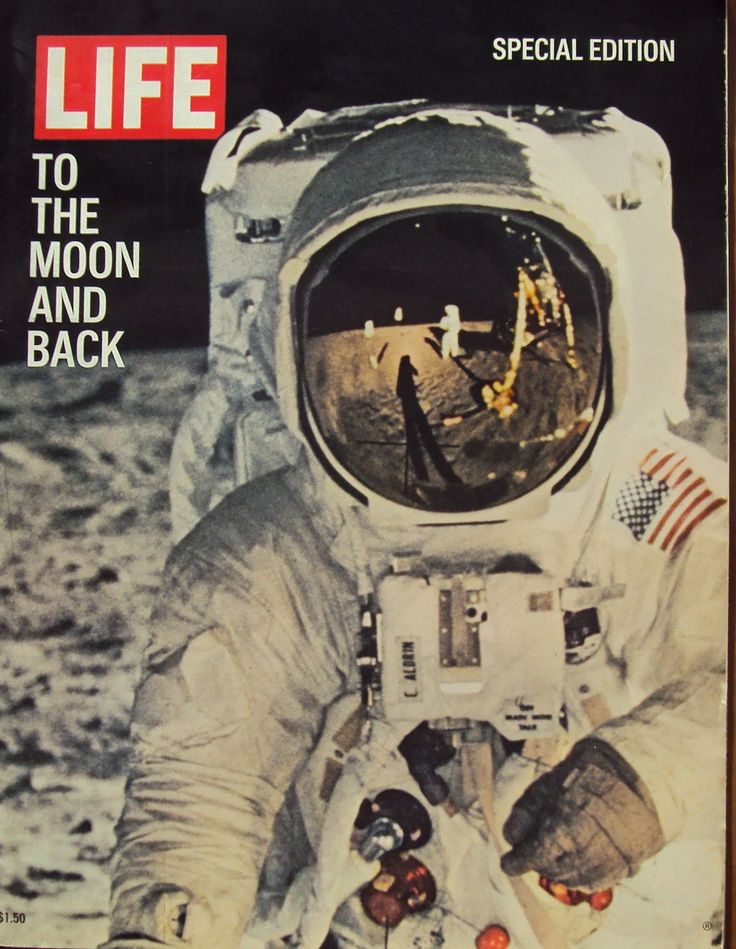
\includegraphics[width=0.9\textwidth]{memories/2.jpg}
\caption{
Map of LaFramboise Island
}
\end{figure}

The days were counting down toward the deadline for removal of the camp.
Memories of the camp include the following.
There was a tipi as a focal point of the camp.
A sacred fire was kept burning all the time.
We took turns helping with the cooking.
Being May the temperatures were cool during the day and cold at night.
The tent I used was our family tent.
I slept in a sleeping bag with extra blankets on a cot but found it difficult to keep warm.
The nearby woods was a source of Morel mushrooms.
I watched people go into the woods and come out with bags of mushrooms.
I walked through the woods wanting to see the Morels that everyone seemed to love.
I only saw a few.
My eyes were not trained to see the mushroom and I likely walked by them by the dozen.

There were afternoon visits to the capital building to observe a hearing regarding the dispute and meet with officials.
There was a threat of a disturbance at night.
At night we took turns watching at the gate where the causeway came onto the island.
One night a car showed up at the far end of the cause way and my memory is that a shot was fired on the mainland side.
Thankfully violence did not break out.

After two weeks I returned to my home with all of its comforts.
The camp eventually disbanded but I'm not sure that the Treaty land was returned to the Oceti Sakowin nation.

A CPT urgent action request.

https://cpt.
org//es/cptnet/1999/04/17/pierre-sd-urgent-action-federal-south-dakota-governments-seeking-expidite-land-tra





